% ===============================
% VoiceNotion Documentation (Supervisor-Compliant Structure)
% ===============================
\documentclass[12pt,a4paper]{report}

% --- Packages ---
\usepackage[utf8]{inputenc}
\usepackage[T1]{fontenc}
\usepackage[french,english]{babel}
\usepackage{graphicx}
\usepackage{float}
\usepackage{hyperref}
\usepackage{enumitem}
% Disable red link borders in contents/figures
\hypersetup{
  hidelinks,
  colorlinks=true,
  linkcolor=black,
  urlcolor=blue,
  citecolor=black
}
\usepackage{geometry}
\usepackage{fancyhdr}
\usepackage[listings]{tcolorbox}
\usepackage{xcolor}
\usepackage{wrapfig}
\usepackage{tikz}
\usepackage{listings}
\usepackage{caption}
\definecolor{voicenotionLightGray}{RGB}{240,240,240}
% Dark background color for code snippets
\definecolor{codebg}{RGB}{30,30,30}
% Global style for all listings
% macros
\newcommand{\resref}[1]{\hyperref[#1]{[\ref*{#1}]}}

\lstset{
  basicstyle=\ttfamily\footnotesize\color{white},
  backgroundcolor=\color{codebg},
  keywordstyle=\color{cyan},
  commentstyle=\color{green!70},
  stringstyle=\color{yellow},
  numbers=left,
  numberstyle=\tiny\color{gray!50},
  breaklines=true,
  columns=fullflexible
}

% Define a simple codebox environment for code snippets
\newtcblisting{codebox}{%
  listing only,
  colback=codebg,
  colframe=codebg!80,
  left=1mm, right=1mm, top=1mm, bottom=1mm,
  boxrule=0.5pt, arc=2pt,
  fonttitle=\bfseries,
  title=Code,
  listing options={%
    basicstyle=\ttfamily\footnotesize\color{white},
    breaklines=true,
    columns=fullflexible,
    keywordstyle=\color{cyan},
    commentstyle=\color{green!70},
    stringstyle=\color{yellow},
    numbers=left,
    numberstyle=\tiny\color{gray!50},
    backgroundcolor=\color{codebg}
  }
}
\geometry{margin=2.5cm}

% --- Title ---
\title{VoiceNotion: Documentation}
\author{BENBOUZID Rima, DOUMAZ Imene}
\date{\today}

\definecolor{coverBorderColor}{RGB}{0,0,0}
\usetikzlibrary{calc}
\begin{document}

% --- Cover Page ---
% \maketitle

% --- Custom Original Cover Page ---
\begin{titlepage}
\thispagestyle{empty}

\begin{tikzpicture}[remember picture,overlay]
  % Draw thick black border around the page with reduced top/bottom margins
  \draw [line width=2pt, coverBorderColor] 
    ($(current page.north west) + (0.8cm,-0.4cm)$) 
    rectangle 
    ($(current page.south east) + (-0.8cm,0.4cm)$);
    
  % Draw inner border - thinner line with reduced top/bottom margins
  \draw [line width=0.5pt, coverBorderColor] 
    ($(current page.north west) + (1.1cm,-0.7cm)$) 
    rectangle 
    ($(current page.south east) + (-1.1cm,0.7cm)$);
\end{tikzpicture}

\begin{center}
    \vspace*{0.1cm}
    {\Large \textbf{République Algérienne Démocratique et Populaire}} \\
    \vspace{0.3cm}
    {\large Ministère de l'Enseignement Supérieur et de la Recherche Scientifique} \\
    \vspace{0.3cm}
    {\large Université M'hamed Bougara - Boumerdès} \\
    \vspace{0.6cm}
    
    
\includegraphics[width=4.5cm]{assets/docs/university_logo.png} \\
    \vspace{0.6cm}
    
    {\large Faculté des Sciences} \\
    \vspace{0.2cm}
    {\large Département d'Informatique} \\
    \vspace{0.6cm}
    
    \begin{tabular}{rl}
        \textbf{Domaine} & : Mathématiques Informatique \\
        \textbf{Filière} & : Informatique \\
        \textbf{Spécialité} & : Développement Web et Infographie \\
    \end{tabular} \\
    
    {\small \textit{N° de l'Arrêté d'habilitation de la spécialité : arrêté n°002 du 03/01/2021}} \\
    \vspace{0.7cm}
    
    {\large \textit{\underline{Mémoire de fin d'études en vu de l'obtention du}}} \\
    {\large \textit{\underline{Diplôme de Licence Professionnelle}}} \\
    \vspace{0.7cm}
    
    {\LARGE \textbf{Thème}} \\
    \vspace{0.6cm}
    
    % Create box with project title matching the reference image
    \begin{tikzpicture}
        \node[draw, rounded corners=15pt, line width=1pt, minimum width=14cm, minimum height=3.5cm] {
            \begin{minipage}{13cm}
                \begin{center}
                    \vspace{-0.5cm}
                    \fontsize{22}{26}\selectfont \textbf{VoiceNotion} \\
                    \fontsize{22}{26}\selectfont \textbf{AI-Based Voice Productivity SaaS Application}
                \end{center}
            \end{minipage}
        };
    \end{tikzpicture}
    \vspace{0.8cm}

    \begin{tabular}{p{8cm}p{6cm}}
        \textbf{Présenté par :} & \textbf{Supervisé par :} \\
        BENHADJER Foudhil Abdellah & CHAOUCHE Ali \\
        SADAOUI Ayoub & \\
        HAFSAOUI Abderahim & \\
    \end{tabular} \\
    \vspace{0.8cm}
    
    {\normalsize Soutenu le \underline{24/06/2024} Devant le jury composé de} \\
    \vspace{0.4cm}
    \begin{tabular}{lll}
        SIACI Redouane & : & Examinateur \\
        HAMMICHE Mokhtar & : & Président \\
    \end{tabular}
\end{center}
\end{titlepage}


% --- Résumé & Abstract ---
% ===============================
% Résumé (French Summary)
% ===============================
\chapter*{Résumé}
\addcontentsline{toc}{chapter}{Résumé}
Ce mémoire présente la conception et le développement de SayNote, une application innovante de prise de notes basée sur la reconnaissance vocale et l’édition par blocs. L’objectif principal est de permettre aux utilisateurs de capturer, organiser et structurer rapidement leurs idées à l’aide de commandes vocales intuitives, tout en offrant une expérience utilisateur moderne et multiplateforme.

Après une étude approfondie des méthodes traditionnelles et des solutions existantes, nous proposons une architecture technique fondée sur les technologies web et mobiles les plus récentes, intégrant des fonctionnalités avancées telles que la transcription vocale intelligente, la gestion flexible des notes et une interface utilisateur épurée. Le projet met également l’accent sur l’accessibilité, la sécurité des données et l’intégration d’une identité visuelle forte.

Les résultats obtenus démontrent la faisabilité et la pertinence de SayNote pour répondre aux besoins actuels des étudiants, professionnels et créateurs de contenu. Ce travail ouvre la voie à de futures améliorations, notamment l’enrichissement des fonctionnalités collaboratives et l’optimisation continue de la reconnaissance vocale.

% ===============================
% Abstract (English Summary)
% ===============================
\chapter*{Abstract}
\addcontentsline{toc}{chapter}{Abstract}
This thesis presents the design and development of VoiceNotion, an innovative note-taking application based on voice recognition and block-based editing. The main objective is to enable users to quickly capture, organize, and structure their ideas using intuitive voice commands, while providing a modern, cross-platform user experience.

After a thorough study of traditional methods and existing solutions, we propose a technical architecture built on the latest web and mobile technologies, integrating advanced features such as intelligent voice transcription, flexible note management, and a streamlined user interface. The project also emphasizes accessibility, data security, and the integration of a strong visual identity.

The results demonstrate the feasibility and relevance of VoiceNotion in meeting the current needs of students, professionals, and content creators. This work paves the way for future improvements, including enhanced collaborative features and ongoing optimization of voice recognition.


% --- Table of Contents, Figures, Tables ---
\tableofcontents
\listoffigures
% \listoftables

% --- General Introduction ---
\chapter*{Introduction générale}
\addcontentsline{toc}{chapter}{Introduction générale}
% Introduction Chapter for VoiceNotion Documentation

% --- Introduction non numérotée ---
\begin{center}
\textbf{\large Introduction du Chapitre}
\end{center}

\noindent
Ce chapitre présente le contexte, les objectifs et la portée du projet VoiceNotion. Il offre une vue d'ensemble sur la motivation derrière l'application, les principales fonctionnalités attendues, ainsi que la structure du document. Le lecteur acquerra une compréhension globale du projet avant d'entrer dans les détails techniques et conceptuels des chapitres suivants.

\thispagestyle{fancy}

\vspace{1cm}

Dans un monde en constante évolution, la technologie est devenue essentielle pour transformer divers secteurs, y compris le domaine de la prise de notes et de la création de documents. Avec l'essor des assistants vocaux et des technologies de reconnaissance vocale, le potentiel d'innovation dans la façon dont nous capturons et organisons nos pensées est immense.

VoiceNotion représente une approche innovante pour capturer, organiser et affiner les pensées principalement par commandes vocales, complétée par un éditeur intuitif basé sur des blocs. L'application vise à être la solution de référence pour les utilisateurs qui valorisent la rapidité, l'efficacité et la flexibilité de la saisie vocale, sans sacrifier les riches capacités d'édition des éditeurs de blocs modernes.

\vspace{0.5cm}

L'idée principale derrière VoiceNotion est de créer une expérience fluide de prise de notes et de création de documents, optimisée pour les appareils mobiles. L'application s'adresse aux étudiants, aux professionnels, aux écrivains et à toute personne ayant besoin de noter rapidement des idées, d'organiser des notes ou de rédiger des documents en déplacement.

\vspace{0.5cm}

La vision de VoiceNotion est de devenir l'application de choix pour ceux qui cherchent à maximiser leur productivité en transformant la parole en contenu structuré et organisé. En combinant la puissance des commandes vocales avec l'organisation intuitive des éditeurs de blocs, VoiceNotion offre une solution innovante aux défis de la prise de notes traditionnelle.

\vspace{1cm}

\section*{Objectifs du projet}
\addcontentsline{toc}{section}{Objectifs du projet}

Les objectifs principaux du projet VoiceNotion sont :

\begin{itemize}
    \item Développer une application mobile entièrement fonctionnelle permettant aux utilisateurs de créer et d'éditer des notes via des commandes vocales.
    \item Implémenter un éditeur basé sur BlockNote.js offrant une expérience d'édition par blocs similaire à Notion.
    \item Assurer une transcription vocale de haute fidélité et une analyse intelligente des intentions de l'utilisateur.
    \item Créer une interface utilisateur intuitive et conviviale optimisée pour les appareils mobiles.
    \item Fournir une application web complémentaire pour une expérience cross-platform complète.
\end{itemize}

\vspace{1cm}

\section*{Portée du document}
\addcontentsline{toc}{section}{Portée du document}

Ce document sert de guide complet pour l'application VoiceNotion, couvrant sa base conceptuelle, son architecture technique, les détails d'implémentation, la conception de l'expérience utilisateur et l'identité visuelle. Il est destiné aux développeurs, designers et parties prenantes impliqués dans le projet, fournissant une compréhension approfondie de la structure et de la fonctionnalité de l'application.

La documentation est organisée en plusieurs chapitres, chacun couvrant un aspect spécifique du développement et de la conception de VoiceNotion :

\begin{itemize}
    \item \textbf{Étude préalable} : Analyse du problème, objectifs du projet et solutions proposées.
    \item \textbf{Planification et conception UX} : Méthodologie de développement, recherche utilisateur et conception du système.
    \item \textbf{Implémentation et développement} : Architecture technique, technologies utilisées et détails d'implémentation.
    \item \textbf{Identité visuelle} : Conception de la marque, éléments visuels et interfaces utilisateur.
\end{itemize}

Ce document servira de référence tout au long du cycle de développement du projet et pourra être utilisé comme base pour la formation, la maintenance et l'évolution future de l'application VoiceNotion. 

% --- Conclusion non numérotée ---
\vspace{1cm}
\begin{center}
\textbf{\large Conclusion du Chapitre}
\end{center}

\noindent
En résumé, ce chapitre introductif a permis de cerner le contexte, les objectifs et la portée du projet VoiceNotion. Il prépare le lecteur à explorer les aspects détaillés de la solution, depuis l'étude préalable jusqu'à la conception, l'implémentation et l'identité visuelle, en fournissant une base solide pour la compréhension du reste de la documentation.

% ===============================
% PART I (unnamed): State of the Art
% ===============================

% --- Chapter 1: Study of the existence ---
\chapter{Étude de l'existant}
% VoiceNotion - Chapitre 2 : Étude de l’existant
% Ce chapitre analyse l’état actuel de la prise de notes et de la gestion d’informations, en s’appuyant sur les pratiques, outils et défis rencontrés par les utilisateurs.

% --- Introduction non numérotée ---
\begin{center}
\textbf{\large Introduction du Chapitre}
\end{center}

\noindent
Ce chapitre dresse un état des lieux des pratiques actuelles de prise de notes et de gestion d’informations, en identifiant les méthodes utilisées, les difficultés rencontrées et les limites des solutions existantes. L’objectif est de comprendre le contexte et les besoins réels des utilisateurs avant toute proposition de solution.

\section{Introduction}

La prise de notes et la gestion d’informations sont des activités essentielles pour de nombreux profils : étudiants, professionnels, créatifs, etc. Malgré la diversité des outils disponibles, de nombreux utilisateurs rencontrent encore des obstacles dans l’organisation, la fiabilité et l’accessibilité de leurs notes. Ce chapitre propose une analyse détaillée de l’existant afin de mettre en lumière les défis à relever.

\section{Contexte de la prise de notes}

La prise de notes intervient dans des contextes variés : réunions, cours, brainstorming, déplacements, etc. Les utilisateurs cherchent à capturer rapidement des idées, à structurer des informations, et à pouvoir y accéder facilement sur différents supports (papier, ordinateur, mobile). L’évolution des usages montre une transition progressive du papier vers les outils numériques, sans pour autant résoudre tous les problèmes liés à la gestion efficace des notes.

\section{Méthodes actuelles de gestion des notes et informations}

La gestion des notes repose aujourd’hui sur une grande diversité de méthodes et d’outils, qu’on peut regrouper en plusieurs catégories :

\subsection{Prise de notes manuelle}
\begin{itemize}
    \item Utilisation de carnets, feuilles volantes, post-its.
    \item Facilité d’accès mais risque élevé de perte, de désorganisation ou d’oubli.
    \item Difficulté à rechercher ou à partager l’information.
\end{itemize}

\subsection{Outils numériques classiques}
\begin{itemize}
    \item Logiciels de traitement de texte (Word, Google Docs), tableurs, emails.
    \item Avantages : sauvegarde, partage, édition facile.
    \item Limites : structure peu adaptée à la prise de notes rapide, fragmentation des fichiers, manque de synchronisation multi-appareils.
\end{itemize}

\subsection{Applications spécialisées de prise de notes}
\begin{itemize}
    \item Applications comme Notion, Evernote, OneNote, Google Keep, Apple Notes.
    \item Fonctions avancées : organisation hiérarchique, recherche, étiquettes, synchronisation cloud, prise de notes vocale.
    \item Limitations relevées par les utilisateurs :
    \begin{itemize}
        \item Transcription vocale parfois imprécise, surtout en environnement bruyant ou multilingue.
        \item Fonctionnalités inégales entre versions web et mobile.
        \item Interface parfois complexe ou non adaptée à l’usage mobile rapide.
        \item Problèmes de synchronisation ou de perte de données occasionnelle.
        \item Dépendance à la connexion internet pour certaines fonctions.
        \item Gestion des historiques ou des versions parfois limitée.
    \end{itemize}
\end{itemize}

\subsection{Organisation et archivage}
\begin{itemize}
    \item Utilisation de dossiers, tags, favoris, et moteurs de recherche pour classer et retrouver l’information.
    \item Archivage manuel ou automatisé, mais risque de fragmentation et de perte de contexte.
    \item Difficulté à maintenir une organisation cohérente sur le long terme.
\end{itemize}

\section{Défis et limitations de l’existant}

Malgré la richesse des outils disponibles, plusieurs défis majeurs persistent :
\begin{itemize}
    \item \textbf{Efficacité limitée :} La prise de notes rapide et structurée reste difficile, en particulier lors de situations de mobilité ou de multitâche.
    \item \textbf{Précision et fiabilité :} Les erreurs de transcription, la perte de données ou les problèmes de synchronisation peuvent nuire à la confiance dans l’outil.
    \item \textbf{Fragmentation de l’information :} La multiplication des supports et applications conduit à une dispersion des notes, rendant leur gestion et leur recherche complexes.
    \item \textbf{Accessibilité et ergonomie :} Les interfaces ne sont pas toujours adaptées à tous les usages (mobile, desktop, voix), ce qui limite l’adoption ou l’efficacité.
    \item \textbf{Confidentialité et dépendance :} La dépendance à des services cloud externes soulève des questions de confidentialité et de pérennité des données.
\end{itemize}

\section{Problématique}

Face à ces limites, de nombreux utilisateurs expriment le besoin d’une solution qui soit à la fois rapide, fiable, accessible sur tous leurs appareils, et capable d’organiser l’information sans effort supplémentaire. La question centrale devient alors : comment concevoir un outil de prise de notes qui réponde réellement aux attentes de mobilité, de fiabilité, d’ergonomie et de sécurité des utilisateurs modernes ?

\section{Conclusion}

Ce chapitre a permis de dresser un panorama complet des pratiques et outils actuels de prise de notes, en mettant en évidence leurs forces et faiblesses. Cette analyse de l’existant constitue le socle sur lequel s’appuiera la réflexion autour d’une solution innovante, présentée dans le chapitre suivant.

% --- Conclusion non numérotée ---
\vspace{1cm}
\begin{center}
\textbf{\large Conclusion du Chapitre}
\end{center}

\noindent
En conclusion, l’étude de l’existant révèle des besoins réels et non totalement satisfaits en matière de prise de notes et de gestion d’informations. Les prochaines sections proposeront une réponse adaptée à ces enjeux, en s’appuyant sur les constats établis ici.
\section{Problématiques}

La prise de notes traditionnelle, qu'elle soit manuscrite ou numérique, présente plusieurs défis majeurs que nous avons identifiés à travers notre recherche et nos observations:

\subsection{Limites de la saisie manuelle}

La saisie manuelle de notes, que ce soit à l'aide d'un stylo et papier ou d'un clavier, présente plusieurs inconvénients:

\begin{itemize}
    \item \textbf{Vitesse limitée:} La vitesse de frappe moyenne (40-60 mots par minute) ou d'écriture manuscrite (10-30 mots par minute) est souvent insuffisante pour capturer efficacement des informations lors de réunions, conférences ou sessions de brainstorming rapides.
    
    \item \textbf{Fatigue et inconfort:} La saisie prolongée peut entraîner une fatigue des mains et des poignets, particulièrement sur les appareils mobiles où les claviers virtuels offrent une expérience sous-optimale.
    
    \item \textbf{Attention divisée:} Le fait de devoir se concentrer sur la saisie divise l'attention de l'utilisateur, réduisant sa capacité à écouter activement ou à participer pleinement à une discussion.
\end{itemize}

\subsection{Accessibilité réduite}

Les méthodes traditionnelles de prise de notes présentent des obstacles d'accessibilité significatifs:

\begin{itemize}
    \item \textbf{Mobilité réduite:} Les personnes souffrant de limitations motrices peuvent éprouver des difficultés considérables avec la saisie manuelle.
    
    \item \textbf{Situations multi-tâches:} De nombreux contextes (conduite, marche, exercice) rendent la saisie manuelle difficile voire impossible.
    
    \item \textbf{Barrières linguistiques:} Pour les utilisateurs non natifs d'une langue, la saisie écrite peut présenter des difficultés supplémentaires par rapport à l'expression orale.
\end{itemize}

\subsection{Complexité de structuration}

L'organisation et la structuration efficaces des notes représentent un défi majeur:

\begin{itemize}
    \item \textbf{Effort post-capture:} La transformation de notes brutes en contenu structuré et organisé nécessite souvent un effort supplémentaire considérable.
    
    \item \textbf{Rigidité des formats:} De nombreuses applications de prise de notes offrent des structures rigides qui limitent la flexibilité et l'adaptabilité aux différents types de contenu.
    
    \item \textbf{Courbe d'apprentissage:} Les éditeurs avancés comme Notion requièrent un investissement initial en temps pour maîtriser leurs fonctionnalités.
\end{itemize}

% \begin{figure}[H]
%     \centering
%     \includegraphics[width=0.8\textwidth]{../assets/docs/note_taking_challenges.png}
%     \caption{Défis de la prise de notes traditionnelle}
%     \label{fig:note_taking_challenges}
% \end{figure}




% \begin{figure}[H]
%     \centering
%     \includegraphics[width=0.7\textwidth]{../assets/docs/voicenotion_concept.png}
%     \caption{Concept de VoiceNotion: fusion entre commandes vocales et éditeur par blocs}
%     \label{fig:voicenotion_concept}
% \end{figure}

























% \begin{figure}[H]
%     \centering
%     \includegraphics[width=0.8\textwidth]{../assets/docs/voicenotion_advantages.png}
%     \caption{Avantages comparatifs de VoiceNotion}
%     \label{fig:voicenotion_advantages}
% \end{figure}

\section{Conclusion}


% --- Conclusion non numérotée ---
\vspace{1cm}
\begin{center}
\textbf{\large Conclusion du Chapitre}
\end{center}

\noindent
En conclusion, cette étude préalable a permis de cerner les besoins, les défis et les opportunités du secteur de la prise de notes. Cette étude préalable met en évidence les besoins, les défis et les opportunités du secteur de la prise de notes. Elle conclut sur l'importance d'une réflexion approfondie pour répondre aux attentes des utilisateurs, sans anticiper sur la solution à proposer.

% --- Chapter 2: Description of the proposed solution ---
\chapter{Description de la solution proposée}
% ===============================
% Chapter: Description de la solution proposée
% ===============================

\section*{Introduction}
\addcontentsline{toc}{section}{Introduction}
Cette section présente la solution VoiceNotion, conçue pour révolutionner la prise de notes grâce à la voix, l’intelligence artificielle et une expérience utilisateur moderne.

\section{Présentation générale de VoiceNotion}
VoiceNotion est une application multiplateforme (web et mobile) dédiée à la prise de notes structurées, à l’édition intuitive et à la productivité augmentée. Elle s’adresse aux étudiants, professionnels et créateurs de contenu souhaitant capturer, organiser et partager leurs idées de manière fluide et efficace.

Après cette présentation générale, le diagramme de cas d’utilisation principal ci-dessous illustre les interactions majeures entre l’utilisateur et l’application :

% --- Placeholder: Use case diagram ---
\begin{figure}[H]
    \centering
    %\includegraphics[width=0.7\textwidth]{assets/docs/use-case-diagram.png}
    \fbox{\parbox{0.6\textwidth}{\centering Placeholder pour le diagramme de cas d’utilisation}}
    \caption{Diagramme de cas d’utilisation principal}
    \label{fig:use-case}
\end{figure}

\section{Fonctionnalités principales}
\begin{itemize}
    \item \textbf{Prise de notes et édition par la voix :} Créez, structurez et modifiez vos notes simplement en parlant.
    \item \textbf{Assistant IA intégré :} Posez des questions, obtenez des résumés, suggestions ou reformulations instantanées.
    \item \textbf{Éditeur par blocs flexible :} Organisez vos contenus en blocs modulables, avec une hiérarchie infinie et des options de formatage avancées.
    \item \textbf{Synchronisation temps réel et hors-ligne :} Accédez à vos notes sur tous vos appareils, même sans connexion internet.
    \item \textbf{Recherche et partage instantanés :} Trouvez n’importe quelle information en quelques secondes et partagez vos notes en un clic.
    \item \textbf{Personnalisation avancée :} Thèmes clair/sombre, icônes, mise en page adaptable à vos préférences.
\end{itemize}

Pour illustrer l’expérience utilisateur, la maquette suivante donne un aperçu de l’interface principale de VoiceNotion :

% --- Placeholder: UI mockup ---
\begin{figure}[H]
    \centering
    %\includegraphics[width=0.6\textwidth]{assets/docs/ui-mockup.png}
    \fbox{\parbox{0.5\textwidth}{\centering Placeholder pour la maquette d’interface utilisateur}}
    \caption{Maquette de l’interface utilisateur de VoiceNotion}
    \label{fig:ui-mockup}
\end{figure}

\section{Architecture technique (aperçu)}
VoiceNotion repose sur une architecture cloud moderne, combinant une interface web (Next.js/React), une application mobile (React Native/Expo), et un backend sécurisé (Supabase, PostgreSQL). L’intégration de l’API Gemini permet une transcription vocale précise et contextuelle.

Pour conclure cette section, le schéma ci-dessous présente une vue d’ensemble de l’architecture technique de la solution :

% --- Placeholder: Global architecture diagram ---
\begin{figure}[H]
    \centering
    %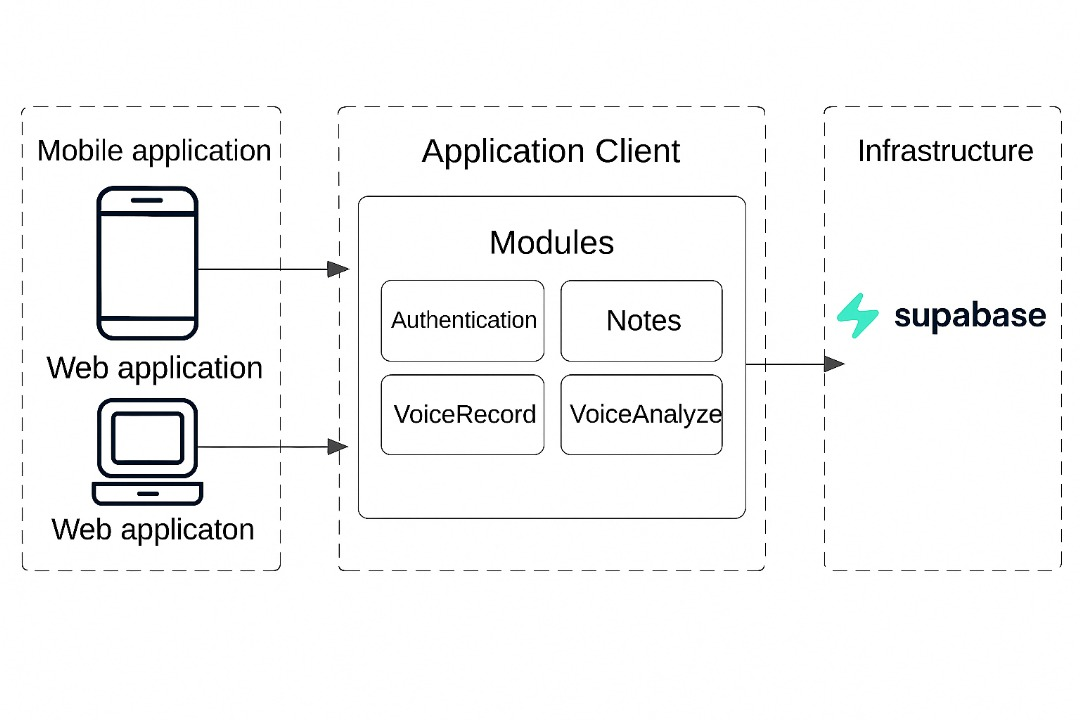
\includegraphics[width=0.8\textwidth]{assets/docs/global-architecture.png}
    \fbox{\parbox{0.7\textwidth}{\centering Placeholder pour le schéma d’architecture globale}}
    \caption{Schéma d’architecture globale de VoiceNotion}
    \label{fig:global-architecture}
\end{figure}

\section{Cas d’utilisation principaux}
VoiceNotion répond à une variété de scénarios d’utilisation courants :
\begin{itemize}
    \item \textbf{Prise de notes en réunion :} Capturer rapidement les points clés, décisions et actions lors de réunions professionnelles ou associatives.
    \item \textbf{Notes d’étude :} Structurer des résumés de cours, fiches de révision et annotations pour les étudiants.
    \item \textbf{Saisie d’idées spontanées :} Enregistrer une idée, une inspiration ou une tâche à tout moment grâce à la saisie vocale instantanée.
    \item \textbf{Édition collaborative :} Partager et modifier des notes en temps réel avec d’autres utilisateurs pour faciliter le travail d’équipe.
    \item \textbf{Gestion de listes et d’organisateurs personnels :} Créer des listes de tâches, agendas ou carnets de bord personnalisés.
\end{itemize}

\section{Sécurité et confidentialité}
La sécurité et la confidentialité des données sont au cœur de la conception de VoiceNotion :
\begin{itemize}
    \item \textbf{Authentification sécurisée :} Utilisation de Supabase pour une gestion robuste des comptes et des accès.
    \item \textbf{Chiffrement des données :} Les notes et informations sensibles sont stockées de manière chiffrée côté serveur.
    \item \textbf{Respect de la vie privée :} Aucune donnée personnelle n’est partagée avec des tiers sans consentement explicite.
    \item \textbf{Conformité RGPD :} Les utilisateurs peuvent exporter ou supprimer leurs données à tout moment, conformément aux exigences européennes.
\end{itemize}

\section{Accessibilité et inclusivité}
VoiceNotion vise à offrir une expérience accessible à tous les utilisateurs :
\begin{itemize}
    \item \textbf{Commandes vocales avancées :} Navigation et édition complètes via la voix, réduisant la dépendance au clavier ou à l’écran tactile.
    \item \textbf{Mode hors-ligne :} Accès et modification des notes sans connexion internet, avec synchronisation automatique lors du retour en ligne.
    \item \textbf{Interface adaptable :} Thèmes clair/sombre, tailles de police ajustables et contrastes optimisés pour les personnes malvoyantes.
    \item \textbf{Compatibilité multi-appareils :} Utilisation fluide sur ordinateurs, tablettes et smartphones.
\end{itemize}

\section{Comparaison avec les solutions existantes}
Bien que des applications comme Notion ou Evernote proposent des fonctionnalités avancées, VoiceNotion se distingue par :
\begin{itemize}
    \item \textbf{Intégration native de la saisie et édition vocale :} La voix est au centre de l’expérience, permettant une prise de notes plus rapide et naturelle.
    \item \textbf{Assistant IA embarqué :} Génération de résumés, réponses contextuelles et suggestions automatiques directement dans l’application.
    \item \textbf{Simplicité d’usage :} Interface épurée, prise en main rapide et fonctionnalités essentielles accessibles en un clic.
    \item \textbf{Synchronisation temps réel et mode hors-ligne complet :} Continuité de l’expérience utilisateur, même sans réseau.
\end{itemize}

\section{Limites actuelles et évolutions prévues}
Malgré ses atouts, VoiceNotion présente certaines limites actuelles :
\begin{itemize}
    \item \textbf{Reconnaissance vocale perfectible :} La précision peut varier selon l’accent ou l’environnement sonore ; des améliorations sont prévues via l’intégration de nouveaux modèles.
    \item \textbf{Fonctionnalités collaboratives en développement :} Les options de coédition et de gestion avancée des partages seront enrichies dans les prochaines versions.
    \item \textbf{Personnalisation limitée :} De nouveaux thèmes, widgets et options de configuration sont à l’étude pour mieux répondre aux besoins variés des utilisateurs.
    \item \textbf{Intégrations tierces :} L’ajout de connecteurs avec d’autres outils (calendriers, gestion de tâches, etc.) est planifié.
\end{itemize}

\section*{Conclusion}
\addcontentsline{toc}{section}{Conclusion}
VoiceNotion propose une solution innovante et complète pour la prise de notes moderne, alliant puissance technologique, simplicité d’utilisation et adaptabilité aux besoins des utilisateurs.


% ===============================
% PART II (unnamed): Contribution
% ===============================

% --- Chapter 1: Conception (includes Visual Identity) ---
\chapter{Conception}
% ===============================
% Conception (inclut Identité Visuelle)
% ===============================

% --- Introduction non numérotée ---
\begin{center}
\textbf{\large Introduction du Chapitre}
\end{center}

\noindent
Ce chapitre présente la démarche de conception de SayNote, en détaillant la méthodologie de planification, la conception UX, la modélisation, ainsi que l'identité visuelle de la marque. L'objectif est d'expliquer comment les choix de conception soutiennent la vision, l'expérience utilisateur et la cohérence de la marque.

% ===============================
% Section 1: Planification et UX
% ===============================
\section{Planification et conception UX}
\input{SayNote_planification_ux}

% ===============================
% Section 2: Identité Visuelle
% ===============================
\section{Identité visuelle}
\input{SayNote_visual_identity}

% --- Conclusion non numérotée ---
\vspace{1cm}
\begin{center}
\textbf{\large Conclusion du Chapitre}
\end{center}

\noindent
Ce chapitre a mis en lumière l'importance d'une conception réfléchie, de la planification à l'identité visuelle. L'intégration de l'UX et du branding garantit une expérience utilisateur optimale et une marque forte, éléments essentiels pour le succès et la différenciation du projet SayNote.



% --- Chapter 2: Implementation ---
\chapter{Implémentation}
% VoiceNotion Implementation and Development Chapter
% Chapter 3 of the VoiceNotion documentation

% --- Introduction non numérotée ---
\begin{center}
\textbf{\large Introduction du Chapitre}
\end{center}

\noindent
Ce chapitre présente en détail l'implémentation technique de VoiceNotion, en mettant l'accent sur l'architecture, les choix technologiques et les défis rencontrés lors du développement. Le lecteur découvrira comment les différentes composantes s'articulent pour offrir une expérience de prise de notes vocale innovante, performante et sécurisée.

\section{Introduction}
Cette partie du mémoire est consacrée à l'implémentation et au développement de l'application VoiceNotion. Nous allons détailler l'architecture technique, les technologies utilisées, et les différentes composantes de notre solution. VoiceNotion est une application de prise de notes vocale qui combine une interface web responsive et une application mobile, toutes deux partageant une base de données commune et des fonctionnalités similaires.

Notre approche de développement a été guidée par les principes de modularité, de réutilisabilité et d'expérience utilisateur fluide. Nous avons adopté des technologies modernes pour garantir la performance, la sécurité et l'évolutivité de notre solution.

\section{Architecture globale}
L'architecture de VoiceNotion est construite autour d'une approche multi-plateforme avec un backend commun. Cette architecture permet de maintenir une expérience utilisateur cohérente tout en optimisant le développement pour chaque plateforme.

% Explication brève avant chaque figure
\noindent
\textit{La figure suivante illustre un aspect clé de l'architecture ou de l'implémentation technique du système.}
\begin{figure}[H]
\centering
\textit{Image manquante: Architecture globale de VoiceNotion}
\caption{Architecture globale de VoiceNotion. Ce schéma technique présente la structure générale du système, mettant en avant l'intégration entre le frontend, le backend et les services tiers.}
\label{fig:global-architecture}
\end{figure}

\subsection{Composants principaux}
\begin{itemize}
    \item \textbf{Application Web}: Développée avec Next.js et React, offrant une interface responsive et optimisée pour les navigateurs desktop et mobiles.
    \item \textbf{Application Mobile}: Construite avec React Native et Expo, permettant un déploiement natif sur iOS et Android.
    \item \textbf{Backend}: Utilisant Supabase comme solution Backend-as-a-Service (BaaS) pour l'authentification, la base de données, et le stockage.
    \item \textbf{API Gemini}: Intégration de l'API Gemini de Google pour la reconnaissance vocale et le traitement des commandes.
\end{itemize}

\subsection{Flux de données}
Le flux de données dans VoiceNotion suit un modèle client-serveur avec synchronisation en temps réel:
\begin{enumerate}
    \item L'utilisateur interagit avec l'application (web ou mobile)
    \item Les requêtes sont envoyées au backend Supabase via des API sécurisées
    \item Les données sont stockées dans une base de données PostgreSQL
    \item Les mises à jour sont synchronisées en temps réel entre les appareils grâce aux abonnements Supabase
\end{enumerate}

\section{Environnement de developpement}
\subsection{Materiels}
Le developpement de VoiceNotion a ete realise sur les equipements suivants:
\begin{itemize}
    \item MacBook Pro M1 (16GB RAM, 512GB SSD)
    \item iPhone 13 Pro (pour les tests iOS)
    \item Samsung Galaxy S21 (pour les tests Android)
    \item iPad Pro (pour les tests de la version tablette)
\end{itemize}

\subsection{Logiciels et outils de developpement}

\subsubsection{Visual Studio Code}
\begin{wrapfigure}{r}{0.3\textwidth}
    \centering
    
\includegraphics[width=0.25\textwidth]{assets/docs/vscode.png}
\end{wrapfigure}
Visual Studio Code est un editeur de code source leger mais puissant qui s'execute sur votre bureau et est disponible pour Windows, macOS et Linux. Il est fourni avec un support integre pour JavaScript, TypeScript et Node.js et dispose d'un riche ecosysteme d'extensions pour d'autres langages et environnements de developpement.

Visual Studio Code a ete notre IDE principal pour le developpement de VoiceNotion. Nous avons utilise plusieurs extensions pour ameliorer notre productivite:

\begin{itemize}
    \item ESLint: Pour la verification du code JavaScript/TypeScript
    \item Prettier: Pour le formatage automatique du code
    \item React Developer Tools: Pour le debogage des composants React
    \item Tailwind CSS IntelliSense: Pour l'autocompletion des classes Tailwind
    \item GitLens: Pour une meilleure integration avec Git
\end{itemize}

\subsubsection{GitHub}
\begin{wrapfigure}{r}{0.3\textwidth}
    \centering
    
\includegraphics[width=0.25\textwidth]{assets/docs/github.png}
\end{wrapfigure}
GitHub est une plateforme de developpement collaboratif basee sur Git, un systeme de controle de version distribue. Il est largement utilise par les developpeurs pour heberger, gerer et partager des projets de developpement de logiciels.

Sur GitHub, les developpeurs peuvent creer des depots pour stocker leur code source, collaborer avec d'autres developpeurs sur des projets, suivre et gerer les problemes, et faciliter le processus de developpement via des fonctionnalites comme les pull requests, les actions, et plus encore.

Pour VoiceNotion, nous avons utilise GitHub pour:
\begin{itemize}
    \item Gestion du code source avec branches pour chaque fonctionnalite
    \item Organisation du travail d'equipe via les issues et les projets
    \item Integration continue avec GitHub Actions
    \item Revue de code via les pull requests
    \item Documentation du projet dans le wiki et le README
\end{itemize}

\subsubsection{TypeScript}
\begin{wrapfigure}{r}{0.3\textwidth}
    \centering
    
\includegraphics[width=0.25\textwidth]{assets/docs/typescript.png}
\end{wrapfigure}
TypeScript est un sur-ensemble de JavaScript developpe par Microsoft qui ajoute des types statiques optionnels au langage. Il est concu pour le developpement d'applications a grande echelle et se compile en JavaScript standard.

Les avantages de TypeScript que nous avons exploites dans VoiceNotion:
\begin{itemize}
    \item Langage type qui permet de detecter les erreurs lors de la compilation
    \item Compilation en differentes versions ECMAScript a partir de la version 3
    \item De nombreux outils disponibles et une integration parfaite avec VS Code
    \item Un langage oriente objet avec l'introduction du typage, de l'heritage et des notions de public et private
    \item La transition du JavaScript vers TypeScript peut se faire progressivement
    \item La transition inverse tres simple grace a la transpilation en ECMAScript
\end{itemize}

TypeScript nous a permis de developper un code plus robuste et plus maintenable, particulierement important pour une application comme VoiceNotion qui necessite une gestion complexe des interactions utilisateur et des donnees.

\subsubsection{Zod}
\begin{wrapfigure}{r}{0.3\textwidth}
    \centering
    
\includegraphics[width=0.25\textwidth]{assets/docs/logo_zod.png}
\end{wrapfigure}
Zod est une bibliotheque de validation de schemas axee sur TypeScript. Elle offre une API puissante et expressive pour definir et valider des schemas de donnees. 

Avec Zod, nous pouvons facilement definir des regles de validation complexes pour differents types de donnees tels que les chaines de caracteres, les nombres, les tableaux, les objets, et bien d'autres. Il prend en charge des fonctionnalites avancees telles que la validation conditionnelle, les messages d'erreur personnalises et la composition de schemas.

Zod favorise le typage fort et l'inference de types, ce qui en fait un choix ideal pour les projets TypeScript. Il s'integre egalement parfaitement avec des frameworks et des bibliotheques populaires comme React et Express. 

Dans VoiceNotion, nous utilisons Zod pour:
\begin{itemize}
    \item Valider les donnees des formulaires utilisateur
    \item Verifier l'integrite des donnees provenant de l'API
    \item Generer des types TypeScript a partir des schemas de validation
    \item Assurer la coherence des donnees entre le frontend et le backend
\end{itemize}

\subsubsection{Tests}
\begin{wrapfigure}{r}{0.3\textwidth}
    \centering
    
\includegraphics[width=0.25\textwidth]{assets/docs/jest.png}\\
    \vspace{0.5cm}
    
\includegraphics[width=0.25\textwidth]{assets/docs/cypress.png}
\end{wrapfigure}
Pour assurer la qualite et la fiabilite de notre application, nous avons mis en place une strategie de tests complete avec Jest et Cypress.

\textbf{Jest} est un framework de test JavaScript concu pour assurer la correction de n'importe quel code JavaScript. Jest est complet et facile a configurer, et nous l'avons utilise pour les tests unitaires et d'integration.

\textbf{Cypress} est un framework de test end-to-end qui nous permet de tester notre application comme le ferait un utilisateur reel. Il offre une experience de test fiable, rapide et facile a comprendre.

Notre approche de test comprend:
\begin{itemize}
    \item Tests unitaires pour les fonctions et composants individuels
    \item Tests d'integration pour verifier les interactions entre composants
    \item Tests end-to-end pour simuler les parcours utilisateur complets
    \item Tests d'accessibilite pour garantir que l'application est utilisable par tous
\end{itemize}

\section{Outils de conception et design}

\subsection{Figma}
\begin{wrapfigure}{r}{0.3\textwidth}
    \centering
    
\includegraphics[width=0.25\textwidth]{assets/docs/figma.png}
\end{wrapfigure}
Figma est un outil de conception d'interface utilisateur base sur le cloud qui permet aux equipes de collaborer en temps reel. Il est devenu notre outil principal pour la conception de l'interface utilisateur et la creation de prototypes interactifs. Il nous a permis de:

\begin{itemize}
    \item Creer des wireframes et des maquettes haute fidelite
    \item Concevoir un systeme de design coherent avec des composants reutilisables
    \item Collaborer en temps reel sur les designs
    \item Tester les interactions via des prototypes cliquables
    \item Generer des specifications pour les developpeurs
\end{itemize}

L'interface intuitive de Figma et ses fonctionnalites avancees ont grandement facilite le processus de conception, permettant a notre equipe de travailler efficacement meme a distance.

% Explication brève avant chaque figure
\noindent
\textit{La figure suivante illustre un aspect clé de l'architecture ou de l'implémentation technique du système.}
\begin{figure}[H]
\centering

\includegraphics[width=0.9\textwidth]{assets/docs/figma_design_system.png}
\caption{Systeme de design VoiceNotion dans Figma}
\label{fig:figma-design}
\end{figure}

\subsection{Adobe Illustrator}
\begin{wrapfigure}{r}{0.3\textwidth}
    \centering
    
\includegraphics[width=0.25\textwidth]{assets/docs/illustrator.png}
\end{wrapfigure}
Adobe Illustrator est un logiciel de creation graphique et de dessin vectoriel largement utilise dans l'industrie du design. Il offre un large eventail d'outils et de fonctionnalites qui permettent de creer des illustrations, des logos, des icones, des graphiques et d'autres elements visuels de haute qualite. 

Illustrator utilise des vecteurs pour creer des images, ce qui signifie que les dessins peuvent etre redimensionnes et modifies sans perte de qualite. Il prend en charge la creation de formes, le trace de courbes, l'application de couleurs et de degrades, la manipulation des calques et bien plus encore.

Nous avons utilise Adobe Illustrator pour creer les elements graphiques vectoriels de notre identite visuelle:

\begin{itemize}
    \item Logo VoiceNotion et ses variantes
    \item Icones personnalisees
    \item Illustrations pour le site web et l'application
    \item Materiel marketing (bannieres, visuels pour reseaux sociaux)
\end{itemize}

% Explication brève avant chaque figure
\noindent
\textit{La figure suivante illustre un aspect clé de l'architecture ou de l'implémentation technique du système.}
\begin{figure}[H]
\centering
\textit{Image manquante: Création des éléments graphiques avec Adobe Illustrator}
\caption{Creation des elements graphiques avec Adobe Illustrator}
\label{fig:illustrator-assets}
\end{figure}

\subsection{Adobe Photoshop}
\begin{wrapfigure}{r}{0.3\textwidth}
    \centering
    
\includegraphics[width=0.25\textwidth]{assets/docs/photoshop.png}
\end{wrapfigure}
Adobe Photoshop est un logiciel de retouche d'image et de creation graphique largement utilise dans le domaine de la conception, de la photographie et du multimedia. Il offre une gamme complete d'outils et de fonctionnalites avances pour manipuler et ameliorer les images.

Avec Photoshop, nous avons effectue des retouches precises, ajuste la luminosite et le contraste, corrige les couleurs, supprime des objets indesirables, et cree des compositions complexes pour notre application. Cet outil nous a ete particulierement utile pour:

\begin{itemize}
    \item Retoucher les captures d'ecran de l'application
    \item Creer des mockups realistes pour presentations
    \item Preparer des images optimisees pour le web et les applications mobiles
    \item Creer des elements graphiques complexes combines avec Illustrator
\end{itemize}

\section{Backend et services cloud}

\subsection{Supabase}
\begin{wrapfigure}{r}{0.3\textwidth}
    \centering
    
\includegraphics[width=0.25\textwidth]{assets/docs/logo_supabase.png}
\end{wrapfigure}
Supabase est une solution Backend-as-a-Service (BaaS) open-source qui offre une alternative a Firebase. Cette plateforme nous offre:

\begin{itemize}
    \item Une base de donnees PostgreSQL performante et evolutive
    \item Un systeme d'authentification securise avec plusieurs methodes de connexion
    \item Des API RESTful et GraphQL generees automatiquement
    \item Des fonctionnalites de temps reel pour la synchronisation des donnees
    \item Un stockage de fichiers integre
\end{itemize}

Nous avons choisi Supabase pour sa flexibilite, sa scalabilite et sa compatibilite avec PostgreSQL, ce qui nous permet de beneficier d'une base de donnees relationnelle complete sans avoir a gerer l'infrastructure sous-jacente. L'authentification integree et les fonctionnalites en temps reel ont egalement considerablement accelere notre developpement.

Avec Supabase, nous avons pu implementer rapidement des fonctionnalites essentielles comme la synchronisation des notes entre appareils, la gestion des utilisateurs et le stockage des fichiers multimedia associes aux notes.

% Explication brève avant chaque figure
\noindent
\textit{La figure suivante illustre un aspect clé de l'architecture ou de l'implémentation technique du système.}
\begin{figure}[H]
\centering
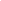
\includegraphics[width=0.8\textwidth]{assets/docs/supabase_dashboard.png}
\caption{Dashboard Supabase pour VoiceNotion}
\label{fig:supabase-dashboard}
\end{figure}

\begin{codebox}{Configuration Supabase}
\begin{lstlisting}
// lib/supabase.ts
import { createClient } from '@supabase/supabase-js';

// Recuperation des variables d'environnement
const supabaseUrl = process.env.NEXT_PUBLIC_SUPABASE_URL!;
const supabaseAnonKey = process.env.NEXT_PUBLIC_SUPABASE_ANON_KEY!;

// Creation et export du client Supabase
export const supabase = createClient(supabaseUrl, supabaseAnonKey);
\end{lstlisting}
\end{codebox}

\subsection{Prisma}
\begin{wrapfigure}{r}{0.3\textwidth}
    \centering
    \textit{Logo Prisma manquant}
\end{wrapfigure}
Prisma est un ORM (Object-Relational Mapping) moderne, mais conçu de manière très différente de ce qui se fait actuellement dans l'industrie. En général, les ORM sont des bibliothèques qui font correspondre les tables de votre base de données aux classes du langage que vous utilisez pour écrire votre programme.

Prisma, quant à lui, est une boîte à outils de base de données complète. En plus, Prisma ne souffre pas des nombreux problèmes qui sont communément associés aux ORM traditionnels. L'équipe estime en effet que l'approche des ORM traditionnels conduit à de nombreux problèmes causés par le décalage d'impédance objet-relationnel.

C'est une situation que la conception de Prisma permet d'éviter. L'un des principaux différenciateurs entre Prisma et un ORM est son fichier de schéma centralisé et son langage de définition de schéma. Ce schéma définit à la fois les modèles de données de l'application et le schéma de la base de données.

\begin{figure}[H]
\centering
\textit{Schéma logique de la base de données pour VoiceNotion. \newline\textit{Ce schéma technique traduit le modèle conceptuel en tables relationnelles pour l'implémentation.}}
\label{fig:prisma-schema}
\end{figure}

Prisma nous permet de:

\textit{La figure suivante illustre un aspect clé de l'architecture ou de l'implémentation technique du système.}
\begin{figure}[H]
\centering
\textit{Image manquante: Page d'inscription du site web}
\caption{Page d'inscription du site VoiceNotion}
\label{fig:web-signup}
\end{figure}

\captionof{figure}{Composant d'authentification}
\label{fig:auth-component}
\begin{lstlisting}[breaklines=true]
// components/AuthForm.tsx
"use client";

import { useState } from "react";
import { supabase } from "@/lib/supabase";
import { Button } from "@/components/ui/Button";
import { Input } from "@/components/ui/Input";

export default function AuthForm({ mode = "login" }) {
  const [email, setEmail] = useState("");
  const [password, setPassword] = useState("");
  const [loading, setLoading] = useState(false);
  const [error, setError] = useState("");
  
  const handleSubmit = async (e) => {
    e.preventDefault();
    setLoading(true);
    setError("");
    
    try {
      if (mode === "login") {
        const { error } = await supabase.auth.signInWithPassword({
          email,
          password,
        });
        if (error) throw error;
      } else {
        const { error } = await supabase.auth.signUp({
          email,
          password,
        });
        if (error) throw error;
      }
    } catch (error) {
      setError(error.message);
    } finally {
      setLoading(false);
    }
  };
  
  return (
    <form onSubmit={handleSubmit} className="space-y-4">
      {error && <div className="p-3 bg-red-100 text-red-700 rounded">{error}</div>}
      
      <div>
        <label htmlFor="email" className="block text-sm font-medium">
          Email
        </label>
        <Input
          id="email"
          type="email"
          value={email}
          onChange={(e) => setEmail(e.target.value)}
          required
        />
      </div>
      
      <div>
        <label htmlFor="password" className="block text-sm font-medium">
          Mot de passe
        </label>
        <Input
          id="password"
          type="password"
          value={password}
          onChange={(e) => setPassword(e.target.value)}
          required
        />
      </div>
      
      <Button type="submit" primary disabled={loading}>
        {loading 
          ? "Chargement..." 
          : mode === "login" ? "Se connecter" : "S'inscrire"}
      </Button>
    </form>
  );
}
\end{lstlisting}

\subsubsection{Tableau de bord}
% Explication brève avant chaque figure
\noindent
\textit{La figure suivante illustre un aspect clé de l'architecture ou de l'implémentation technique du système.}
\begin{figure}[H]
\centering
\textit{Image manquante: Tableau de bord de l'application web}
\caption{Tableau de bord du site VoiceNotion}
\label{fig:web-dashboard}
\end{figure}

\subsubsection{Éditeur de notes}
% Explication brève avant chaque figure
\noindent
\textit{La figure suivante illustre un aspect clé de l'architecture ou de l'implémentation technique du système.}
\begin{figure}[H]
\centering
\textit{Image manquante: Editeur de l'application web}
\caption{Éditeur de notes avec commandes vocales}
\label{fig:web-editor}
\end{figure}

\section{Application mobile}
\subsection{Technologies et outils utilises}

\subsubsection{React Native}
\begin{minipage}{0.7\textwidth}
React Native est un framework de developpement d'applications mobiles cree par Facebook (Meta) qui permet de construire des applications natives pour Android et iOS a partir d'une base de code JavaScript/React commune. Il offre une approche "apprendre une fois, ecrire partout" pour le developpement mobile.

Les principales caracteristiques de React Native qui ont guide notre choix pour VoiceNotion sont:

\begin{itemize}
    \item \textbf{Composants natifs}: React Native compile le code JavaScript en composants natifs, offrant des performances proches des applications natives
    \item \textbf{Partage de code}: Possibilite de partager une grande partie du code entre les plateformes iOS et Android
    \item \textbf{Hot Reloading}: Visualisation instantanee des modifications du code pendant le developpement
    \item \textbf{Communaute active}: Large ecosysteme de bibliotheques et support communautaire
    \item \textbf{Approche declarative}: Interface utilisateur construite de maniere declarative, similaire a React
\end{itemize}

React Native nous a permis de developper l'application mobile VoiceNotion pour iOS et Android a partir d'une seule base de code, tout en offrant une experience utilisateur native et performante sur chaque plateforme.
\end{minipage}%
\hfill
\begin{minipage}{0.25\textwidth}
\centering

\includegraphics[width=0.9\textwidth]{assets/docs/logo_reactnative.png}
\end{minipage}

\begin{codebox}{Configuration du projet React Native}
\begin{lstlisting}
// app.json
{
  "expo": {
    "name": "VoiceNotion",
    "slug": "voicenotion",
    "version": "1.0.0",
    "orientation": "portrait",
    "icon": "./assets/icon.png",
    "userInterfaceStyle": "light",
    "splash": {
      "image": "./assets/splash.png",
      "resizeMode": "contain",
      "backgroundColor": "#ffffff"
    },
    "assetBundlePatterns": ["**/*"],
    "ios": {
      "supportsTablet": true,
      "bundleIdentifier": "com.voicenotion.app"
    },
    "android": {
      "adaptiveIcon": {
        "foregroundImage": "./assets/adaptive-icon.png",
        "backgroundColor": "#ffffff"
      },
      "package": "com.voicenotion.app"
    },
    "plugins": [
      [
        "expo-av",
        {
          "microphonePermission": "Autoriser VoiceNotion a acceder a votre microphone."
        }
      ]
    ]
  }
}
\end{lstlisting}
\end{codebox}

\subsubsection{Expo}
\begin{minipage}{0.7\textwidth}
Expo est une plateforme et un ensemble d'outils construits autour de React Native qui simplifient considerablement le developpement, le test et le deploiement d'applications mobiles. Il offre une approche "batteries included" pour React Native.

Les avantages d'Expo qui ont guide notre choix pour VoiceNotion sont:

\begin{itemize}
    \item \textbf{Configuration simplifiee}: Pas besoin de configurer manuellement le SDK natif d'Android ou iOS
    \item \textbf{Modules preintegres}: Acces a des APIs natives courantes (camera, geolocalisation, etc.) via des modules preconfiguress
    \item \textbf{Expo Go}: Application de test qui permet de visualiser les changements en temps reel sur des appareils physiques
    \item \textbf{EAS (Expo Application Services)}: Services de build, deploiement et mise a jour des applications
    \item \textbf{Over-the-air updates}: Possibilite de deployer des mises a jour sans passer par les App Stores
\end{itemize}

Expo nous a permis d'accelerer considerablement le developpement de l'application mobile VoiceNotion, en simplifiant l'acces aux fonctionnalites natives et en offrant un flux de travail optimise du developpement au deploiement.
\end{minipage}%
\hfill
\begin{minipage}{0.25\textwidth}
\centering

\includegraphics[width=0.9\textwidth]{assets/docs/logo_expo.png}
\end{minipage}

\subsection{Interfaces principales}

\subsubsection{Authentification}
% Explication brève avant chaque figure
\noindent
\textit{La figure suivante illustre un aspect clé de l'architecture ou de l'implémentation technique du système.}
\begin{figure}[H]
    \centering
    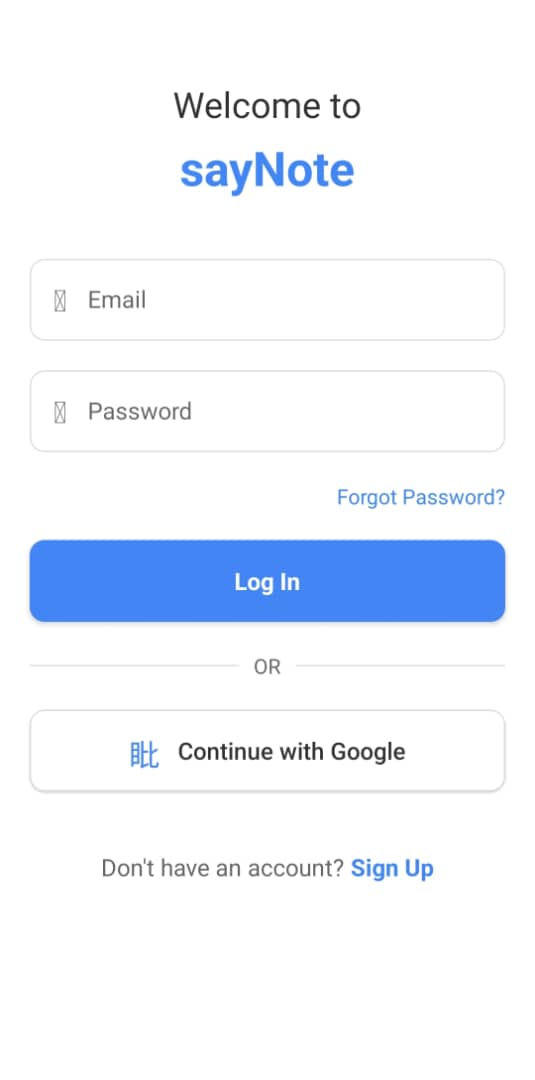
\includegraphics[width=0.4\textwidth]{assets/docs/mobile/login-page.jpeg}
    \hfill
    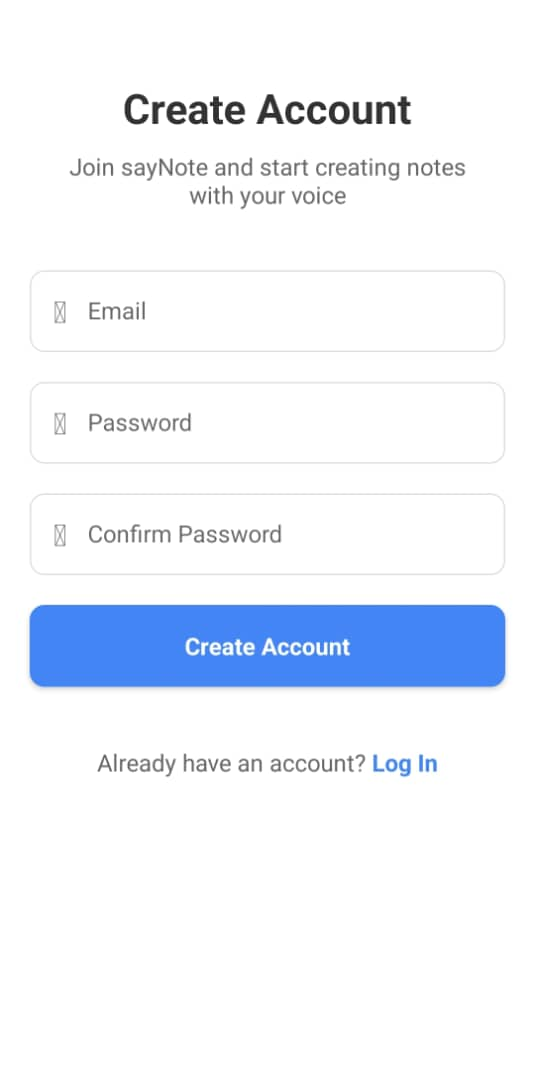
\includegraphics[width=0.4\textwidth]{assets/docs/mobile/create-account-page.jpeg}
    \caption{Écrans de connexion et de création de compte}
    \label{fig:mobile-auth}
\end{figure}

% Explication brève avant chaque figure
\noindent
\textit{La figure suivante illustre un aspect clé de l'architecture ou de l'implémentation technique du système.}
\begin{figure}[H]
    \centering
    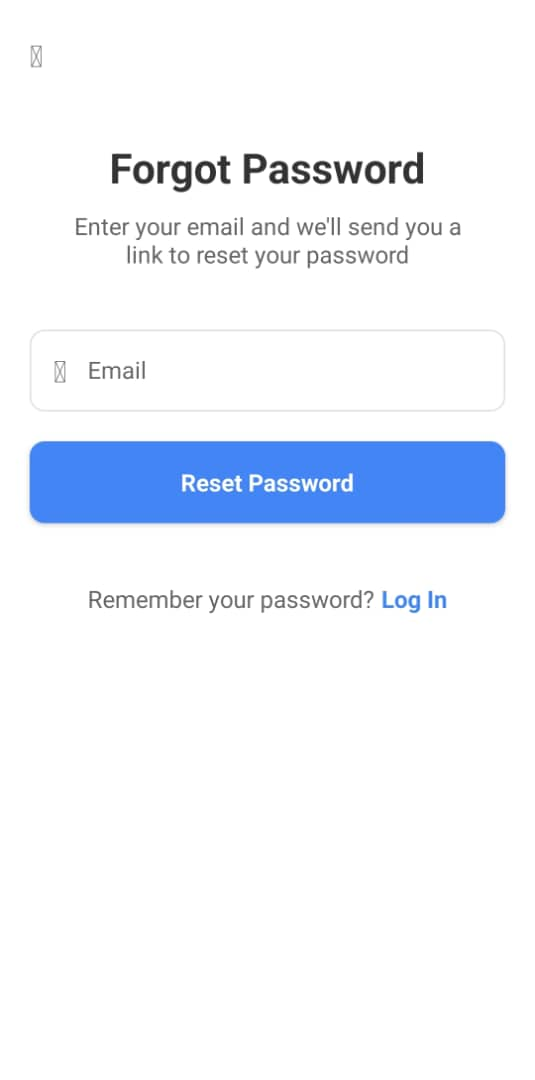
\includegraphics[width=0.4\textwidth]{assets/docs/mobile/forget-password-page.jpeg}
    \caption{Écran de réinitialisation du mot de passe}
    \label{fig:mobile-forgot-password}
\end{figure}

\subsubsection{Navigation et recherche}
% Explication brève avant chaque figure
\noindent
\textit{La figure suivante illustre un aspect clé de l'architecture ou de l'implémentation technique du système.}
\begin{figure}[H]
    \centering
    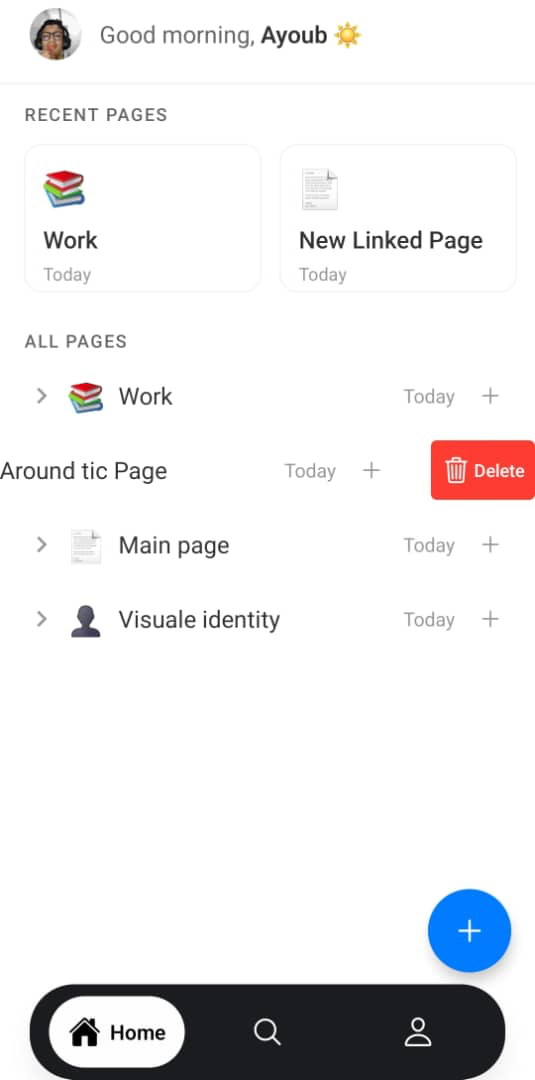
\includegraphics[width=0.4\textwidth]{assets/docs/mobile/home-screen.png}
    \hfill
    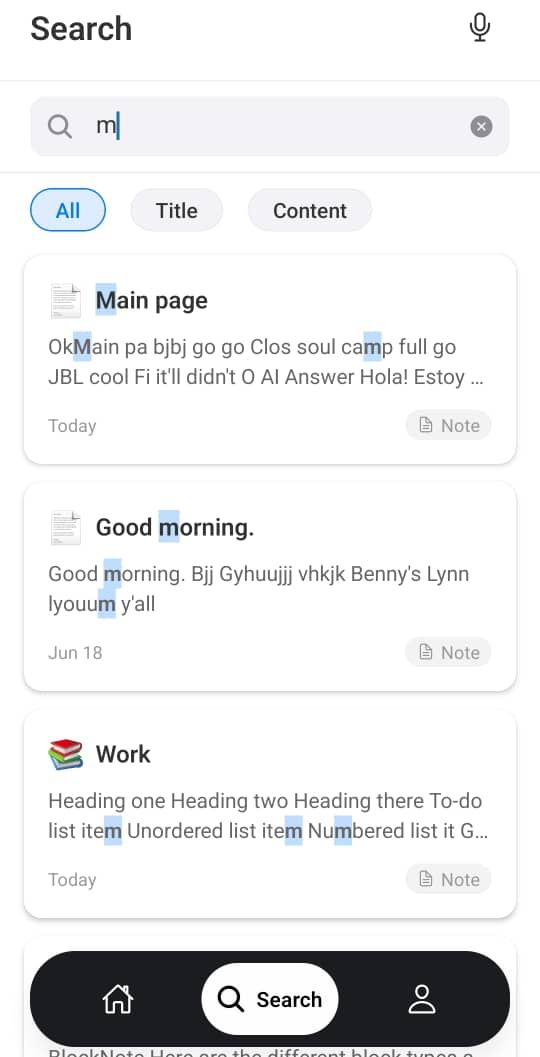
\includegraphics[width=0.4\textwidth]{assets/docs/mobile/search-screeen.png}
    \caption{Écrans d'accueil et de recherche}
    \label{fig:mobile-home-search}
\end{figure}

\subsubsection{Gestion des notes}
% Explication brève avant chaque figure
\noindent
\textit{La figure suivante illustre un aspect clé de l'architecture ou de l'implémentation technique du système.}
\begin{figure}[H]
    \centering
    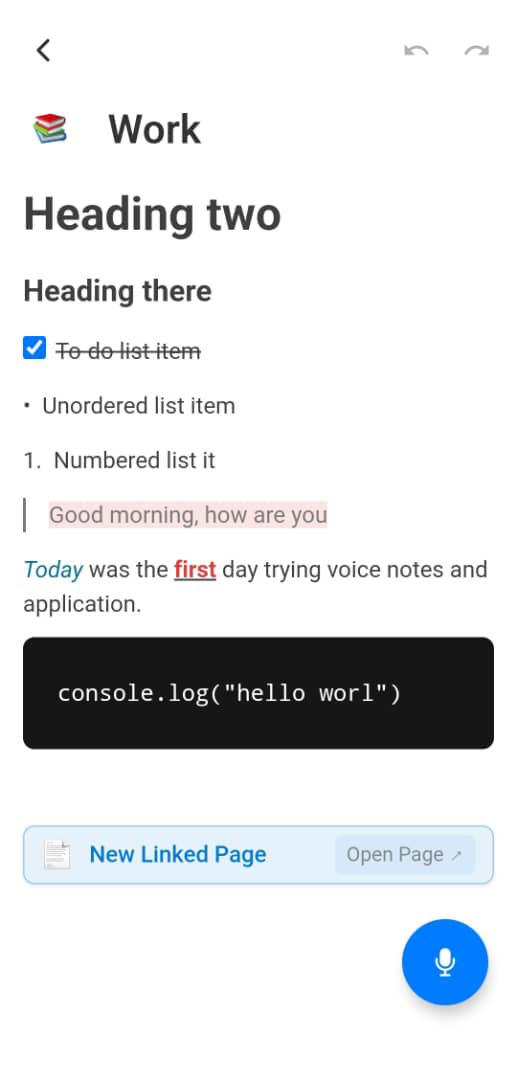
\includegraphics[width=0.4\textwidth]{assets/docs/mobile/note-page.png}
    \hfill
    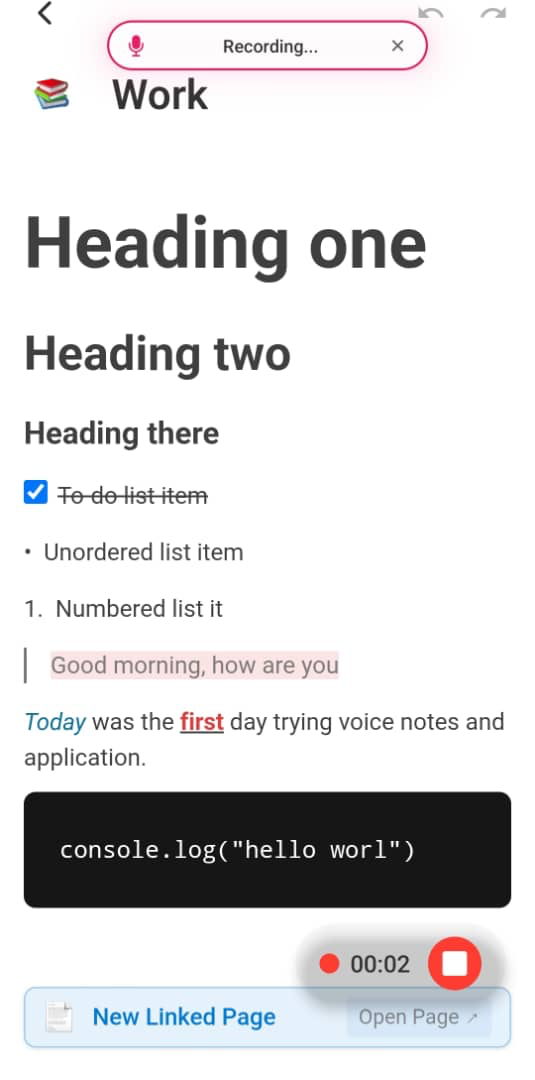
\includegraphics[width=0.4\textwidth]{assets/docs/mobile/note-page-recording.png}
    \caption{Éditeur de notes et enregistrement vocal}
    \label{fig:mobile-editor}
\end{figure}

\subsubsection{Profil utilisateur}
% Explication brève avant chaque figure
\noindent
\textit{La figure suivante illustre un aspect clé de l'architecture ou de l'implémentation technique du système.}
\begin{figure}[H]
    \centering
    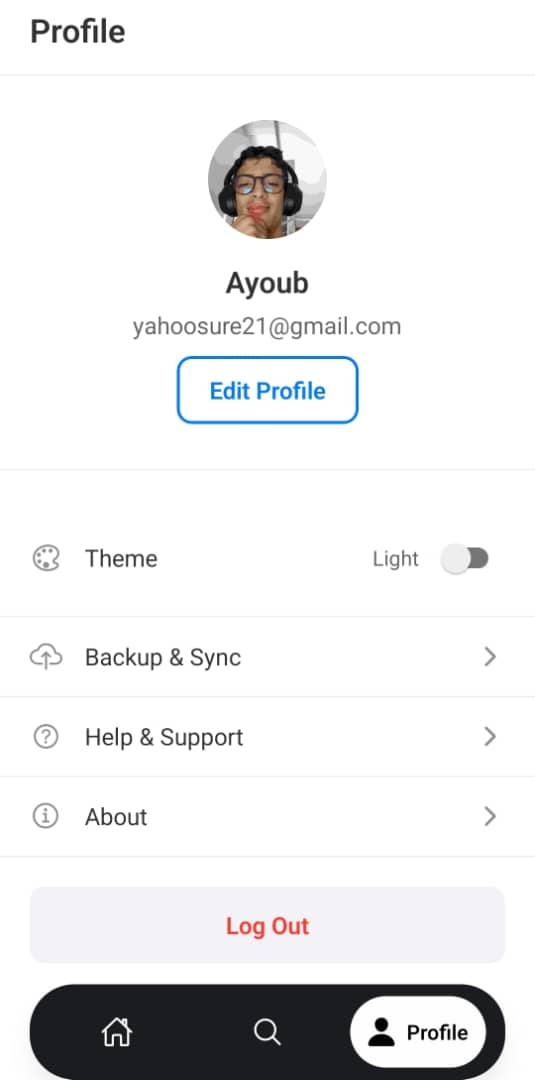
\includegraphics[width=0.4\textwidth]{assets/docs/mobile/profile-screen.png}
    \caption{Écran de profil utilisateur}
    \label{fig:mobile-profile}
\end{figure}

\section{Integration de la reconnaissance vocale}
\subsection{Gemini API}
\begin{minipage}{0.7\textwidth}
L'API Gemini de Google est un modele d'IA multimodal avance qui nous permet d'integrer des capacites de traitement du langage naturel et de comprehension contextuelle dans VoiceNotion. 

Cette API est au coeur de notre fonctionnalite de reconnaissance vocale et nous l'utilisons pour deux fonctions principales:
\begin{itemize}
    \item \textbf{Transcription de la parole en texte (Speech-to-Text)}: Conversion precise de l'audio vocal en texte ecrit
    \item \textbf{Analyse d'intention}: Comprehension et interpretation des commandes vocales pour executer les actions appropriees dans l'application
\end{itemize}

Gemini nous offre plusieurs avantages cles:
\begin{itemize}
    \item \textbf{Comprehension contextuelle}: Capacite a comprendre le contexte des commandes vocales
    \item \textbf{Support multilingue}: Prise en charge de multiples langues pour une utilisation internationale
    \item \textbf{Adaptabilite}: Possibilite d'affiner le modele pour notre cas d'utilisation specifique
    \item \textbf{Integration simple}: API REST facile a integrer dans nos applications web et mobile
\end{itemize}

Grace a Gemini, VoiceNotion peut offrir une experience de dictee vocale naturelle et intuitive, permettant aux utilisateurs de creer et de modifier du contenu a l'aide de commandes vocales complexes.
\end{minipage}%
\hfill
\begin{minipage}{0.25\textwidth}
\centering

\includegraphics[width=0.9\textwidth]{assets/docs/gemini.png}
\end{minipage}

% Explication brève avant chaque figure
\noindent
\textit{La figure suivante illustre un aspect clé de l'architecture ou de l'implémentation technique du système.}
\begin{figure}[H]
\centering
\textit{Image manquante: Diagramme de l'API Gemini}
\caption{Integration de l'API Gemini dans VoiceNotion}
\label{fig:gemini-api}
\end{figure}

\subsection{Flux de traitement des commandes vocales}
Le traitement des commandes vocales dans VoiceNotion suit un flux bien defini:
\begin{enumerate}
    \item Capture de l'audio via le microphone de l'appareil
    \item Conversion de l'audio en texte via l'API Gemini
    \item Analyse de l'intention de la commande (egalement via Gemini)
    \item Execution de l'action correspondante dans l'editeur
    \item Retour visuel et auditif a l'utilisateur
\end{enumerate}

% Explication brève avant chaque figure
\noindent
\textit{La figure suivante illustre un aspect clé de l'architecture ou de l'implémentation technique du système.}
\begin{figure}[H]
\centering
\textit{Image manquante: Flux des commandes vocales}
\caption{Flux de traitement des commandes vocales}
\label{fig:voice-commands-flow}
\end{figure}

\section{Tests et assurance qualite}
\subsection{Strategie de test}
Notre strategie de test pour VoiceNotion comprend plusieurs niveaux:
\begin{itemize}
    \item \textbf{Tests unitaires}: Verification du comportement des composants individuels
    \item \textbf{Tests d'integration}: Validation des interactions entre les differentes parties du systeme
    \item \textbf{Tests end-to-end}: Simulation des parcours utilisateur complets
    \item \textbf{Tests de performance}: Evaluation des temps de reponse et de la consommation de ressources
    \item \textbf{Tests d'accessibilite}: Verification de la conformite aux standards WCAG
\end{itemize}

\subsection{Outils de test}
\begin{itemize}
    \item \textbf{Jest}: Framework de test pour les tests unitaires et d'integration
    \item \textbf{React Testing Library}: Bibliotheque pour tester les composants React
    \item \textbf{Cypress}: Outil pour les tests end-to-end de l'application web
    \item \textbf{Detox}: Framework pour les tests end-to-end de l'application mobile
    \item \textbf{Lighthouse}: Outil pour evaluer les performances et l'accessibilite
\end{itemize}

\section{Deploiement et integration continue}
\subsection{Pipeline CI/CD}
Nous avons mis en place un pipeline d'integration continue et de deploiement continu (CI/CD) pour automatiser le processus de build, test et deploiement:

\begin{itemize}
    \item \textbf{GitHub Actions}: Automatisation des workflows de CI/CD
    \item \textbf{ESLint et Prettier}: Verification de la qualite du code
    \item \textbf{Tests automatises}: Execution des tests a chaque pull request
    \item \textbf{Preview Deployments}: Deploiement de versions de previsualisation pour chaque branche
\end{itemize}

\subsection{Environnements de deploiement}
\begin{itemize}
    \item \textbf{Developpement}: Environnement local pour les developpeurs
    \item \textbf{Staging}: Environnement de preproduction pour les tests
    \item \textbf{Production}: Environnement final accessible aux utilisateurs
\end{itemize}

\subsection{Plateformes de deploiement}
\subsubsection{Digital Ocean}
\begin{minipage}{0.7\textwidth}
Digital Ocean est une solution de service en cloud populaire, dotee d'une infrastructure robuste et offrant de multiples services.

Il est principalement utilise pour l'hebergement d'applications et de sites web et est prefere par les utilisateurs en raison de sa facilite d'utilisation. Les centres de donnees Digital Ocean offrent un haut niveau de securite pour les applications.

Les serveurs prives virtuels ou VPS offerts par Digital Ocean aux utilisateurs sont connus sous le nom de Droplets. Les utilisateurs de la plateforme peuvent gerer leurs applications par le biais d'une interface utilisateur Web ou d'une interface en ligne de commande (CLI).

La plateforme IaaS de Digital Ocean est un choix populaire pour de nombreuses grandes entreprises clientes dans le monde entier en raison de sa fiabilite. Elle permet aux utilisateurs de choisir des parametres tels que les centres de donnees pour les applications, la taille des droplets et la region geographique.

Pour VoiceNotion, nous avons utilise Digital Ocean pour:
\begin{itemize}
    \item Heberger notre base de donnees PostgreSQL de sauvegarde
    \item Gerer des services auxiliaires comme Redis pour la mise en cache
    \item Executer des taches de traitement en arriere-plan
\end{itemize}
\end{minipage}%
\hfill
\begin{minipage}{0.25\textwidth}
\centering
\textit{Logo DigitalOcean manquant}
\end{minipage}

\subsubsection{Nginx}
\begin{minipage}{0.7\textwidth}
Nginx, prononce comme "engine-ex", est un serveur web open-source qui, depuis son succes initial en tant que serveur web, est maintenant aussi utilise comme reverse proxy, cache HTTP, et load balancer.

Nginx a ete cree a l'origine par Igor Sysoev, avec sa premiere sortie publique en octobre 2004. Igor a d'abord concu le logiciel comme une reponse au probleme du C10k, qui est un probleme de performance lie a la gestion de 10.000 connexions simultanees.

Pour VoiceNotion, nous utilisons Nginx pour:
\begin{itemize}
    \item Servir de reverse proxy pour notre application
    \item Gerer le load balancing entre les instances de l'application
    \item Configurer le SSL/TLS pour la securite des communications
    \item Optimiser la diffusion des assets statiques
    \item Mettre en place des regles de cache pour ameliorer les performances
\end{itemize}

Nginx nous a permis d'ameliorer considerablement les performances et la securite de notre application, tout en offrant une flexibilite importante pour la configuration de notre infrastructure.
\end{minipage}%
\hfill
\begin{minipage}{0.25\textwidth}
\centering

\includegraphics[width=0.9\textwidth]{assets/docs/nginx.png}
\end{minipage}

\section{Securite et protection des donnees}
\subsection{Authentification et autorisation}
La securite de VoiceNotion repose sur plusieurs mecanismes:
\begin{itemize}
    \item \textbf{Authentification multi-facteurs}: Pour une securite renforcee des comptes
    \item \textbf{JWT (JSON Web Tokens)}: Pour la gestion des sessions
    \item \textbf{Controle d'acces base sur les roles}: Pour limiter les actions selon le profil utilisateur
\end{itemize}

\subsection{Protection des donnees}
\begin{itemize}
    \item \textbf{Chiffrement des donnees}: En transit (HTTPS) et au repos
    \item \textbf{Anonymisation}: Des donnees utilisees pour l'analyse et l'amelioration du service
    \item \textbf{Sauvegarde reguliere}: Pour prevenir la perte de donnees
\end{itemize}

\subsection{Conformite RGPD}
VoiceNotion est concu dans le respect du Reglement General sur la Protection des Donnees:
\begin{itemize}
    \item \textbf{Consentement explicite}: Pour la collecte et l'utilisation des donnees
    \item \textbf{Droit a l'oubli}: Possibilite de supprimer toutes les donnees utilisateur
    \item \textbf{Portabilite des donnees}: Export des notes dans des formats standards
\end{itemize}

\section{Defis techniques et solutions}
\subsection{Defis rencontres}
Durant le developpement de VoiceNotion, nous avons rencontre plusieurs defis techniques:
\begin{itemize}
    \item \textbf{Precision de la reconnaissance vocale}: Particulierement dans des environnements bruyants
    \item \textbf{Synchronisation en temps reel}: Entre les differents appareils d'un utilisateur
    \item \textbf{Performance de l'editeur}: Avec des documents volumineux
    \item \textbf{Fonctionnement hors ligne}: Gestion des conflits lors de la reconnexion
\end{itemize}

\subsection{Solutions implementees}
\begin{itemize}
    \item \textbf{Filtrage audio}: Algorithmes de reduction du bruit pour ameliorer la reconnaissance vocale
    \item \textbf{Systeme de replication}: Base sur CRDT (Conflict-free Replicated Data Types) pour la synchronisation
    \item \textbf{Virtualisation}: Rendu optimise des longs documents pour maintenir la performance
    \item \textbf{Queue de synchronisation}: Pour gerer les modifications hors ligne et les synchroniser lors de la reconnexion
\end{itemize}

\section{Conclusion}
L'implementation de VoiceNotion a necessite l'integration de nombreuses technologies modernes et la resolution de defis techniques complexes. L'architecture choisie nous a permis de creer une application performante, securisee et evolutive, disponible sur le web et sur mobile.

La combinaison de React, Next.js, React Native et Supabase nous a fourni une base solide pour construire notre solution, tandis que l'integration de l'API Gemini a rendu possible la fonctionnalite centrale de reconnaissance vocale.

Les prochaines etapes de developpement incluront l'amelioration continue de la precision de la reconnaissance vocale, l'ajout de nouvelles fonctionnalites collaboratives, et l'optimisation des performances sur tous les appareils. 

% --- Conclusion non numérotée ---
\vspace{1cm}
\begin{center}
\textbf{\large Conclusion du Chapitre}
\end{center}

\noindent
En résumé, ce chapitre a détaillé l'ensemble des choix techniques, des architectures et des solutions mises en œuvre pour concrétiser VoiceNotion. L'intégration harmonieuse des différentes technologies et la résolution des défis techniques témoignent de la robustesse et de la modernité de l'application. Ces fondations solides ouvrent la voie à de futures évolutions et améliorations, qui seront abordées dans les perspectives finales du document.

% --- General Conclusion ---
\section*{Conclusion générale}
\addcontentsline{toc}{section}{Conclusion générale}
% ===============================
% General Conclusion
% ===============================

Ce mémoire a présenté le processus de conception, de développement et d’implémentation de l’application VoiceNotion. Nous avons analysé les limites des méthodes traditionnelles de prise de notes, défini une solution innovante fondée sur la reconnaissance vocale et l’édition par blocs, puis détaillé la planification, la conception UX, l’identité visuelle et l’implémentation technique.

VoiceNotion se distingue par sa capacité à rendre la prise de notes plus rapide, accessible et flexible pour un large éventail d’utilisateurs. L’architecture technique moderne, l’accent mis sur l’expérience utilisateur et la sécurité des données, ainsi que l’intégration d’une identité visuelle cohérente, constituent les points forts du projet.

Les perspectives d’évolution incluent l’amélioration continue de la reconnaissance vocale, l’ajout de fonctionnalités collaboratives et l’optimisation des performances. Ce travail pose ainsi les bases d’une solution évolutive, adaptée aux besoins futurs en matière de productivité et de gestion de l’information.


% --- Online Resources ---
\chapter*{Ressources en ligne}
\addcontentsline{toc}{chapter}{Ressources en ligne}
Voici une liste non exhaustive de documents et articles de référence consultés durant ce travail :

\begin{enumerate}[label=\arabic*., leftmargin=*]
  \item \href{https://supabase.com/docs}{Supabase Documentation}\label{res:supabase}
  \item \href{https://nextjs.org/docs}{Next.js Documentation}\label{res:nextjs}
  \item \href{https://reactnative.dev/docs/getting-started}{React Native Docs}\label{res:reactnative}
  \item \href{https://docs.expo.dev}{Expo Documentation}\label{res:expo}
  \item \href{https://docs.netlify.com}{Netlify Docs}\label{res:netlify}
  \item \href{https://www.postgresql.org/docs/}{PostgreSQL Official Docs}\label{res:postgresql}
  \item \href{https://figma.com/resources/learn-design}{Figma Design Guides}\label{res:figma}
  \item \href{https://jestjs.io/docs}{Jest Testing Framework Docs}\label{res:jest}
  \item \href{https://docs.cypress.io}{Cypress End-to-End Testing}\label{res:cypress}
  \item \href{https://www.typescriptlang.org/docs}{TypeScript Handbook}\label{res:typescript}
  \item \href{https://nodejs.org/en/docs}{Node.js Documentation}\label{res:node}
  \item \href{https://docs.github.com/en/actions}{GitHub Actions Docs}\label{res:githubactions}
  \item \href{https://jwt.io/introduction}{JWT.io – JSON Web Tokens}\label{res:jwt}
  \item \href{https://owasp.org/www-project-top-ten/}{OWASP Top Ten Security Risks}\label{res:owasp}
  \item \href{https://developer.mozilla.org/en-US/docs/Web/JavaScript/Guide}{MDN JavaScript Guide}\label{res:mdn}
  \item \href{https://cloud.google.com/architecture}{Google Cloud Architecture Center}\label{res:gcp}
  \item \href{https://eslint.org/docs/latest}{ESLint Documentation}\label{res:eslint}
  \item \href{https://prettier.io/docs/en/index.html}{Prettier Formatter Docs}\label{res:prettier}
  \item \href{https://tailwindcss.com/docs}{Tailwind CSS Docs}\label{res:tailwind}
  \item \href{https://testing-library.com/docs/react-testing-library/intro}{React Testing Library}\label{res:reacttestinglibrary}
  \item \href{https://developer.chrome.com/docs/lighthouse/}{Google Lighthouse Docs}\label{res:lighthouse}
  \item \href{https://wix.github.io/Detox/docs/api}{Detox Testing Docs}\label{res:detox}
  \item \href{https://yjs.dev/}{Yjs CRDT Framework}\label{res:crdt}
\end{enumerate}

\end{document}
